% Prepared by Calvin Kent
%
% Assignment Template v19.02
%
%%% 20xx0x/MATHxxx/Crowdmark/Ax
%
\documentclass[12pt]{article} %
\usepackage{CKpreamble}
\usepackage{CKassignment}
\usepackage{tkz-euclide}
\usepackage{physunits}
\usepackage{physics}
\usepackage{lmodern}
\usepackage{microtype}
\usepackage{upgreek}
\usepackage[misc]{ifsym}

%%% Maths and science packages

\usepackage{amsmath,amsthm,amssymb}
\usepackage{pgfplots}
	\usetikzlibrary{
		calc,
		patterns,
		positioning
	}
	\pgfplotsset{
		compat=1.16,
		samples=200,
		clip=false,
		my axis style/.style={
			axis x line=middle,
			axis y line=middle,
			legend pos=outer north east,
			axis line style={
				->,
			},
			legend style={
				font=\footnotesize
			},
			label style={
				font=\footnotesize
			},
			tick label style={
				font=\footnotesize
			},
			xlabel style={
				at={
					(ticklabel* cs:1)
				},
				anchor=west,
				font=\footnotesize,
			},
			ylabel style={
				at={
					(ticklabel* cs:1)
				},
				anchor=west,
				font=\footnotesize,
			},
			xlabel= $t$,
			ylabel=$\vec d (\m \tx{[East]})$
		},
	}
	\tikzset{
		>=stealth
	}

%%% Tables and figures packages

\usepackage{float}
\usepackage{caption}
	\captionsetup{
		format=plain,
		labelfont=bf,
		font=small,
		justification=centering
	}
	
%%% Numbers and sets

\newcommand{\E}{\mathrm{e}}

\newcommand{\tx}[1]{\text{#1}}

\begin{document}
    \pagenumbering{arabic}
    % Start of class settings ...
    \renewcommand*{\coursecode}{Physics Homework} % renew course code
    \renewcommand*{\assgnnumber}{3} % renew assignment number
    \renewcommand*{\submdate}{August 18, 2021} % renew the date
    \renewcommand*{\studentfname}{Abdullah} % Student first name
    \renewcommand*{\studentlname}{Zubair} % Student last name
    %\renewcommand*{\studentnum}{SNumber} % Student number

    \renewcommand\qedsymbol{$\blacksquare$}
    \setfigpath
    % End of class settings 
    \pagestyle{crowdmark}
    \newgeometry{left=18mm, right=18mm, top=22mm, bottom=22mm} % page is set to default values
    \fancyhfoffset[L,O]{0pt} % header orientation fixed
    % End of class settings
    %%% Note to user:
    % CTRL + F <CHANGE ME:> (without the angular brackets) in CKpreamble to specify graphics paths accordingly.
    % The command \circled[]{} accepts one optional and one mandatory argument.
    % Optional argument is for the size of the circle and mandatory argument is for its contents.
    % \circled{A} produces circled A, with size drawn for letter A. \circled[TT]{A} produces circled A with size drawn for TT.
    % https://github.com/CalvinKent/My-LaTeX
    %%%
    % Crowdmark assignment start
\begin{qstn}[1] % qnumber, qname, qpoints
    Answer the following True/False questions (\textbf{Assume [East] is positive})
    \begin{enumerate}
        \item A runner completes a $100\m$ sprint at an average speed of $50 \m / \s$.
        \begin{enumerate}[label = (\alph*)]
            \item The time it took to complete the race was $10$\s. (T / F)
            \item If the runner wishes to complete a $1\km$ race in the same amount of time as he completed the $100\m$ race, his average speed must be $500 \m / \s$. (T / F)
        \end{enumerate}
        \item The position v. time plot of a vehicle over the highway was similar to the plot $y = x$.
        \begin{enumerate}[label = (\alph*)]
            \item The vehicle experienced uniform motion (T / F)
            \item The average velocity was positive (T / F)
        \end{enumerate}
        \item The position v. time plot of a vehicle over the highway was similar to the plot $y = -4$
        \begin{enumerate}[label = (\alph*)]
            \item The vehicle experienced uniform motion (T / F)
            \item The vehicle is [East] of the reference point (T / F)
        \end{enumerate}
        \item Two runners compete in a race starting from $(0,0)$, runner $X$ and runner $Y$. Runner $X$ has a Pos v. Time plot similar to $y = 4x$ and Runner $Y$ has a Pos v. Time plot similar to $y = x$.
        \begin{enumerate}[label = (\alph*)]
            \item Runner $Y$ won the race (T / F)
            \item If the race lasted $4$ seconds, then final position vector of Runner $X$ was $\vec d_X = 12\m$[East] (T / F)
        \end{enumerate}

    \end{enumerate}

 \end{qstn}



 \begin{qstn}[2]
    Using the $x-$dimensional coordinate system, and choosing $(x \rightarrow )$ as the positive direction, I decided to track my tour around the area the other day. All position vectors are recorded relative to $(0,0)$. I \emph{began} my journey at $d_1 = + 5\m$, then,
    \begin{itemize}
        \item $\vec d_2 = + 7\m$
        \item $\vec d_3 = -18\m$
        \item $\vec d_4 = +11\m$
    \end{itemize}
    If the tour lasted for $10\Min$, determine my average velocity as well as my average speed over the tour.
 \end{qstn}



\begin{qstn}[3]
    A tourist traverses $412\km[\tx{W}]$ to the Canada starting from UK. From Canada, he traverses $805\km[\tx{E}]$ to Egypt. Finally, from Egypt he traverses $98\km$[\tx{E}] to Saudi Arabia. If the journey took $2 \h$, determine his average velocity as well as his average speed. 
\end{qstn}


\begin{qstn}[4]
    Racer $X$, Racer $Y$ and Racer $Z$ compete in the Grand Motor Sport. Below is position v. time plot for each of the racers, \textcolor{purple}{Racer $X$},\textcolor{red}{Racer $Y$},\textcolor{blue}{Racer $Z$}. Prove that \textcolor{blue}{Racer $Z$} won the race.(Assume that the race lasted for $5$ seconds)
    \begin{figure}[h]
        \centering
        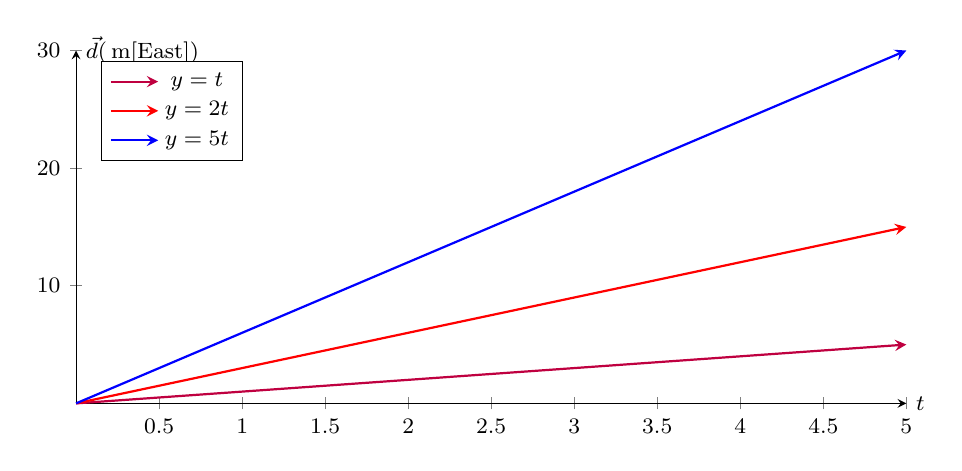
\begin{tikzpicture}
        \begin{axis}[
            my axis style,
            width=\textwidth,
            height=.5\textwidth,
            legend entries={
                $y = t$,
                $y = 2t$,
                $y = 5t$
            },
            legend pos=north west
        ]
        
        \addplot[
            domain=0:5,
            thick,
            purple,
            ->
        ]
        {x};
    
        \addplot[
            domain=0:5,
            thick,
            red,
            ->
        ]
        {3*(x)};
    
        \addplot[
            domain=0:5,
            thick,
            blue,
            ->
        ]
        {6*(x)};
        
        \fill[
            black
        ];
        
        \end{axis}
        \end{tikzpicture}
        \caption{Pos V. Time}
        \label{fig:my-awesome-graph}
    \end{figure}



\end{qstn}


\begin{qstn}[5]
A ball is dropped from a cliff $20\m$[North] relative to the ground. The ball bounces off the ground and reaches a final position $15\m$[South] relative to the cliff. The entire trip took $12$ seconds. Determine,
\begin{enumerate}[label = (\alph*)]
    \item The average velocity of the ball
    \item The average speed of the ball
    \item The Pos v. Time plot of the ball
\end{enumerate}

\end{qstn}


\begin{qstn}[6]
    A sprinter completes a sprint (returning back to his starting position) in $30$ seconds around a circular track with radius $15\m$. Compute the sprinters,
    \begin{enumerate}[label = (\alph*)]
        \item Average speed
        \item Average velocity
    \end{enumerate}


\end{qstn}


\begin{qstn}[7]
    Car $A$ and Car $B$ are about to race each other, however Car $B$ wants to challenge himself by letting car $A$ have a $3$ second head start. If car $A$ has an average speed of $120 \m / \s$, at what average speed must Car $B$ race at in order to tie the race? The length of the race track is $4.2 \km$.
\end{qstn}


\begin{qstn}[8]
    The Robetson's Family are interested in doing business with a particular salesmen. They decide to drive over to Toronto to catch him at his bus stop before he departs. Let us suppose that this bus stop is located at $(0,0)$. The Roberston's mistakenly passed this bus stop, not knowing that the salesmen was at this particular one, and only realized they missed him after having traveled to a position $\vec d = +100\m$ relative to the bus stop, at an average speed of $60 \m / \s$. The \emph{exact} moment they passed him was the moment that his bus started to travel in a direction [West] relative to the bust stop at an average velocity of $50 \m / \s $[\tx{West}]. If at the exact moment the Robertson's had reached the position $\vec d = +100\m$, the salesmen got off at his next stop, at what speed must the Roberston's travel at in order to catch up to him within $30$ seconds?
    \end{qstn}


 



















\end{document}
%   \begin{figure}[H]
%   \centering
%   \includegraphics[width=0.75\linewidth]{p}
%   \caption{caption.\label{fig:}}
%   \end{figure}























